%Start
%required packages and reason
\documentclass[11pt]{article}
\usepackage[a4paper,margin=1in]{geometry}
\usepackage{mathtools} % required for sigma notation
\usepackage{graphicx} %required to load images
\usepackage{amsmath} %required for the matrices
\usepackage{upgreek} %required for Greek symbols
\usepackage{xfrac} %for differentiation symbol
\usepackage{float} %to set the figures exactly where we want,(\figure "[H]")
\usepackage{listings} %to get colorful code in latex
\usepackage{color} %to get a nice color scheme
\usepackage{pythonhighlight} %to make the the python codes nice

%initial headings
\title{EE2703 Assignment 7:  Analysis of Circuits using Laplace Transforms}
\author{Anvith Pabba EE19B070}
\date{15th April 2021}

%begin document
\begin{document}

\maketitle

\section{Introduction}

In this assignment, we use symbolic algebra to analyse filters in the Laplace domain. We use the \textbf{sympy} library and its powerful capabilities to solve the modified nodal equations. We then find the outputs of the filter with different inputs and plot the necessary graphs and analyse our findings.

\section{The Low Pass Filter}
First, we analyse the Low pass filter given below:

\begin{figure}[H]
    \centering
    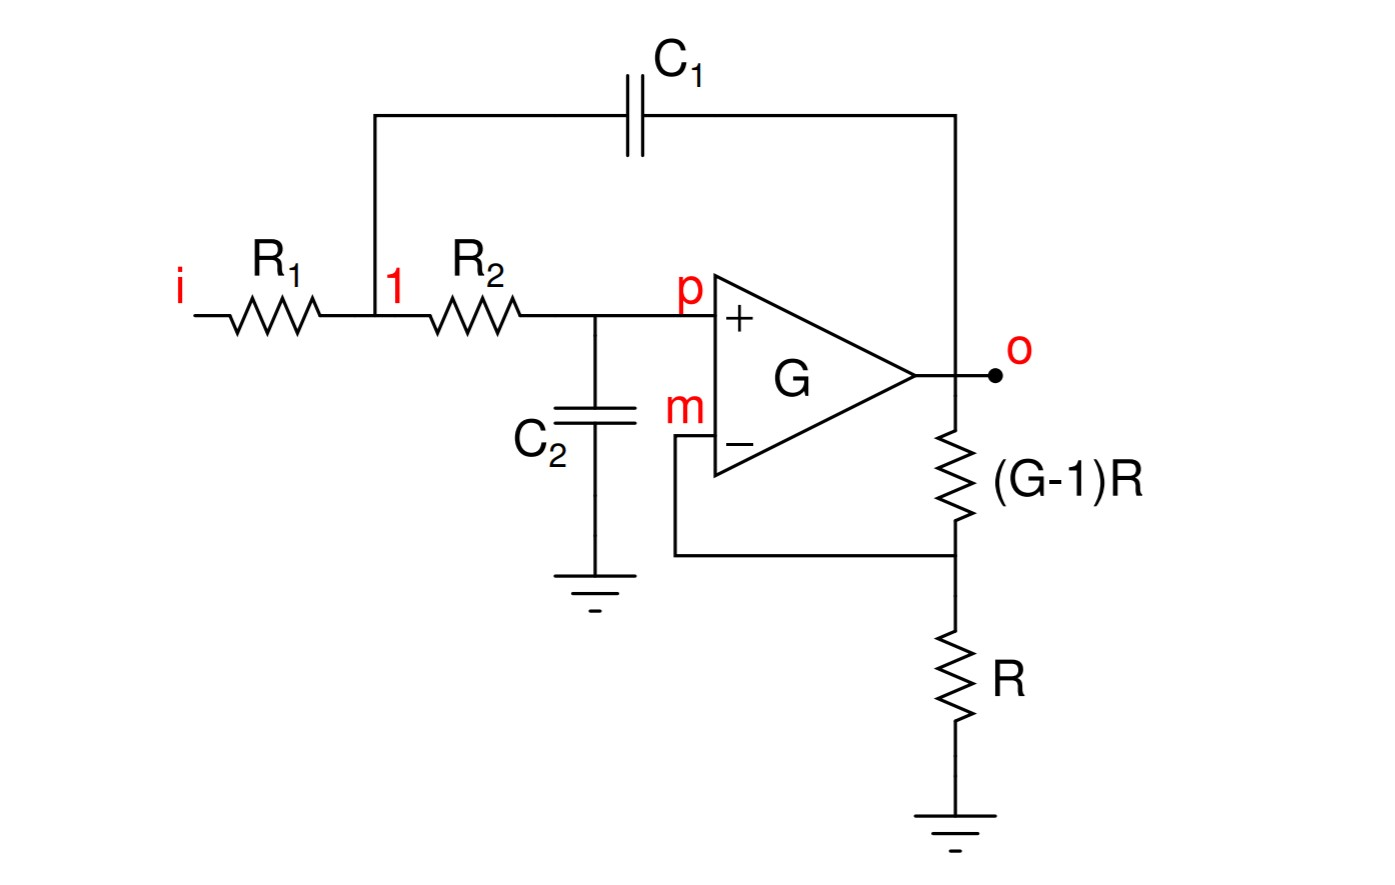
\includegraphics[scale = 1]{LPF.jpg}
    \caption{Diagram of the Low Pass Filter}
\end{figure}

Upon simplifying the equations obtained through modified nodal analysis, we get the following Matrix Equations:

\begin{figure}[H]
    \centering
    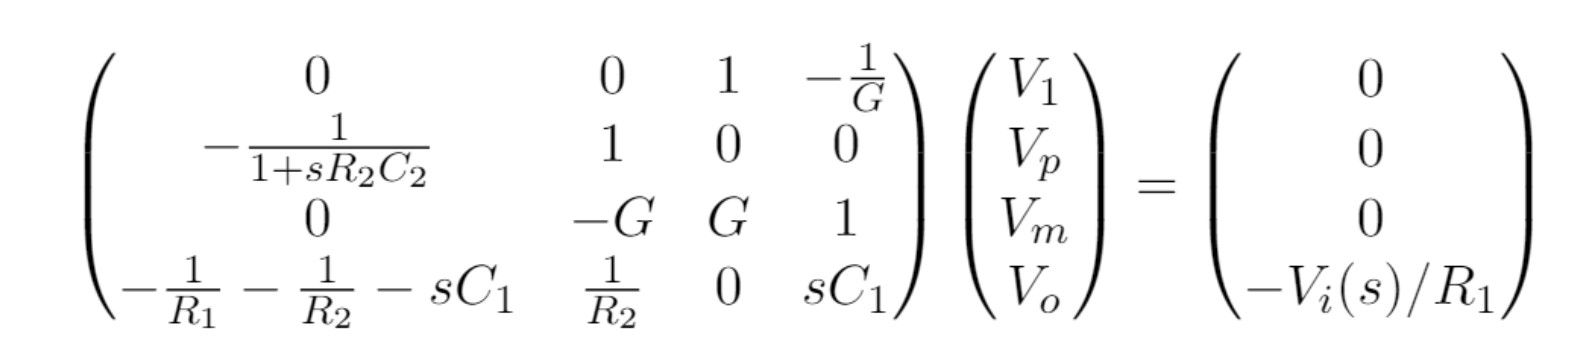
\includegraphics[scale = 1]{LPF_eqns.jpg}
    \caption{Matrix equations for the LPF}
\end{figure}

\subsection{Solving the Equations}
We now define a function that takes in the parameters of the given filter and solves the equations and returns the output voltage (in terms of symbol 's').

\subsubsection{Code:}
\begin{python}
#Defining a Low pass filter in sympy with necessary parameters
def lowpass(R1,R2,C1,C2,G,Vi):
	s=symbols('s')
	# Creating the matrices through nodal analysis then solvng them to get the output
	A=Matrix([[0,0,1,-1/G], [-1/(1+s*R2*C2),1,0,0], [0,-G,G,1], [-1/R1-1/R2-s*C1,1/R2,0,s*C1]])
	b=Matrix([0,0,0,-Vi/R1])
	V=A.inv()*b
	return(A,b,V)
\end{python}

\subsection{Bode plot of Magnitude}
Below we find the Bode magnitude plot of the LPF transfer function:

\begin{figure}[H]
    \centering
    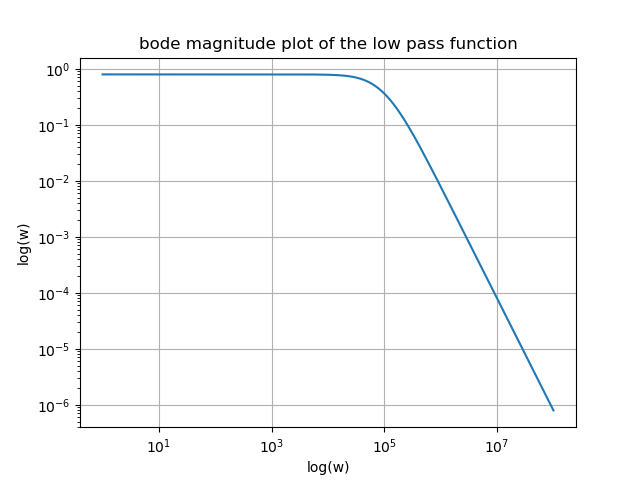
\includegraphics[scale = 1]{Figure_1.png}
    \caption{LPF magnitude bode plot}
\end{figure}



\section{The High Pass Filter}

First, we analyse the High pass filter given below:

\begin{figure}[H]
    \centering
    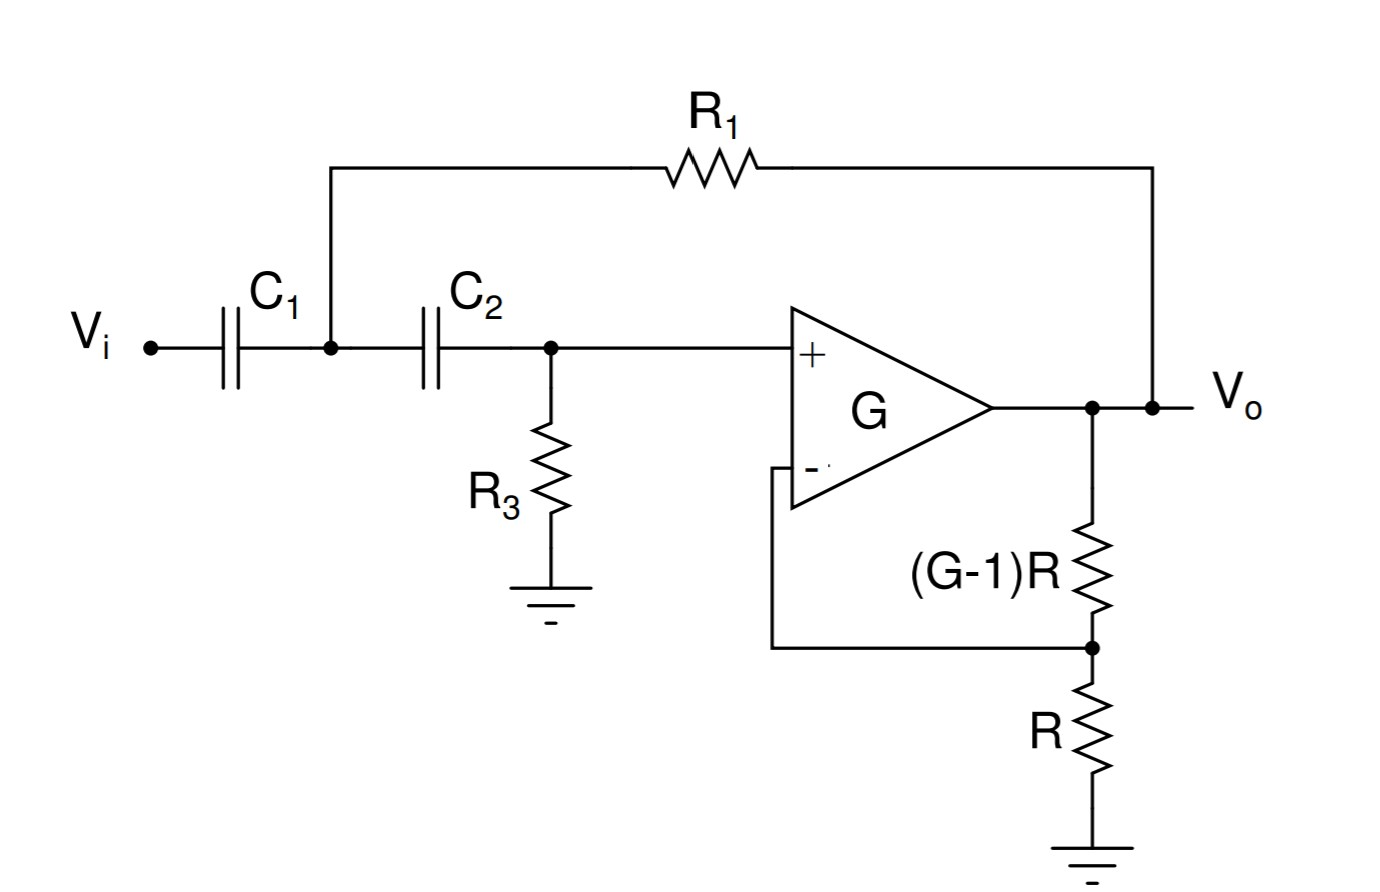
\includegraphics[scale = 1]{HPF.jpg}
    \caption{Diagram of the High Pass Filter}
\end{figure}

Upon simplifying the equations obtained through modified nodal analysis, we get the following Matrix Equations:

\begin{figure}[H]
    \centering
    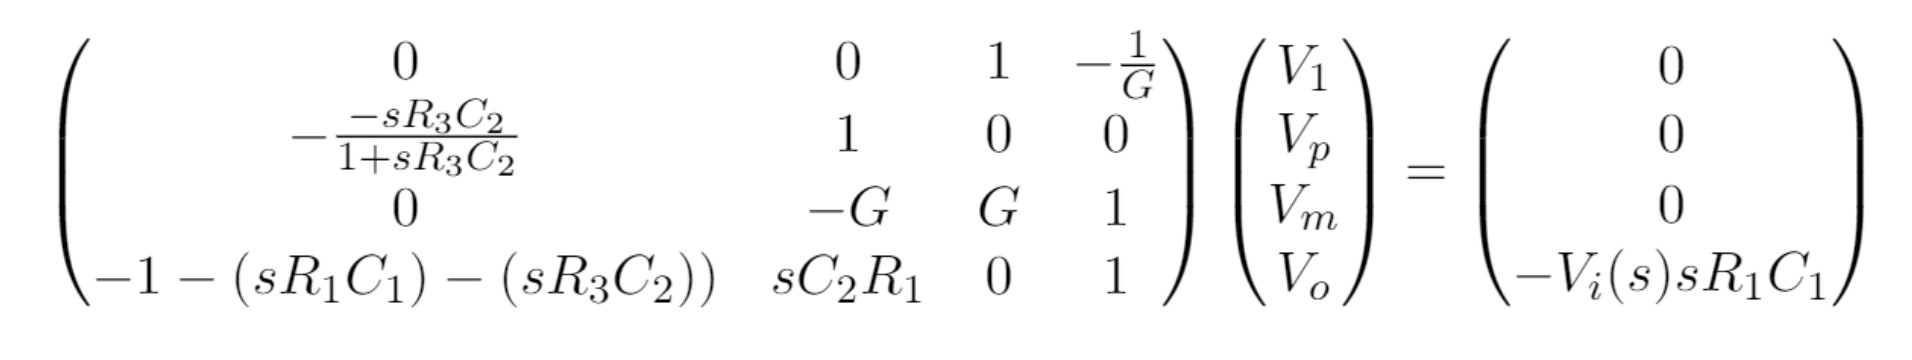
\includegraphics[scale = 0.85]{HPF_eqns.jpg}
    \caption{Matrix equations for the HPF}
\end{figure}


\subsection{Solving the Equations}
We now define a function that takes in the parameters of the given filter and solves the equations and returns the output voltage (in terms of symbol 's').

\subsubsection{Code:}
\begin{python}
#Defining a High pass filter in sympy with necessary parameters

def highpass(R1,R3,C1,C2,G,Vi):
    s = symbols("s")
	# Creating the matrices through nodal analysis then solvng them to get the output
    A = Matrix([[0,-1,0,1/G],[s*C2*R3/(s*C2*R3+1),0,-1,0],[0,G,-G,1],[-s*C2-1/R1-s*C1,0,s*C2,1/R1]])
    b = Matrix([0,0,0,-Vi*s*C1])
    V = A.inv()*b
    return A,b,V
\end{python}


\subsection{Bode plot of Magnitude}
Below we find the Bode magnitude plot of the HPF transfer function:

\begin{figure}[H]
    \centering
    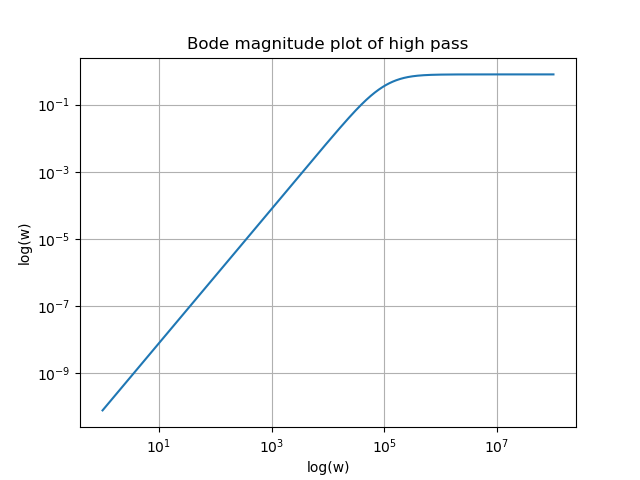
\includegraphics[scale = 1]{Figure_5.png}
    \caption{HPF magnitude bode plot}
\end{figure}

\section{changing a sympy syntax into a scipy acceptable syntax:}
We do this through simple arithmetic manipulations present in the sympy toolkit. We create a function that converts any expression with a sympy variable \textbf{s} into a scipy transfer function. The function is given by: \textbf{sympy\_to\_H\_lti()}

\subsection{Code:}
\begin{python}
#converts an equation containing sympy variables into a function that scipy accepts
def sympy_to_H_lti(sympy_func,s):
	s=symbols('s')
	n,d = fraction(sympy_func)	#getting the numerator and denominator
	num_c = Poly(n,s).all_coeffs()	#getting the coeff
	den_c = Poly(d,s).all_coeffs()
	numf = p.array(num_c, dtype=float)	#converting the arrays into numpy arrays
	denf = p.array(den_c, dtype=float)
	H = sp.lti(numf,denf)	#creating the lti systems transfer response
	return(H)
\end{python}

\section{The Assignment}

\subsection{Question 1: Step response of the LPF}
To do this, we simply change the input function in the formula. As it is a step function, we use the following as the input.
\begin{equation}
    V_i(s) = \frac{1}{s}
\end{equation}

The response we get is from using the \textbf{lambdify} and the \textbf{sp.impulse} commands.

\subsubsection{Code:}
\begin{python}
#Question 1:

#step impulse response, Vi(s) = 1/s
A,b,V1=lowpass(10000,10000,1e-9,1e-9,1.586,1/s)
Vo1 = V1[3]
w = p.logspace(0,8,801)
ss=1j*w
hf1=lambdify(s,Vo1,'numpy')
v=hf1(ss)
H1 = sympy_to_H_lti(Vo1,s)

#plotting the magnitude plot of the step response of the low pass filter
plot_display(w,abs(v),'w','magnitude','Magnitude bode plot of step response of low pass filter','log','log')

t,y=sp.impulse(H1,None,p.linspace(0,0.001,1000))
plot_display(t,y,'t','y','step response of low pass filter','linear','linear')
\end{python}

\subsubsection{Magnitude plot of the transfer function}
\begin{figure}[H]
    \centering
    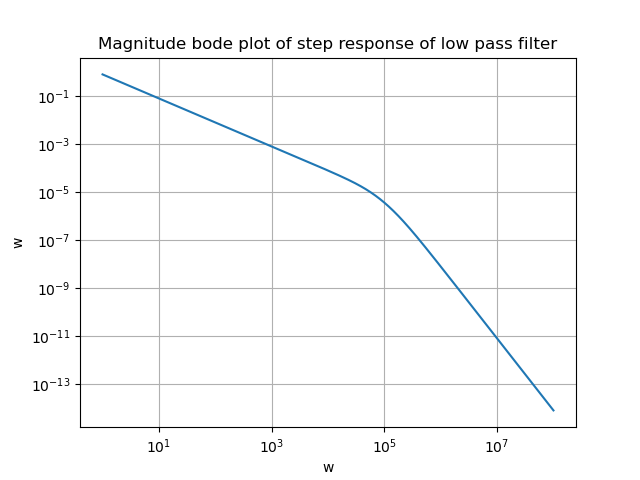
\includegraphics[scale = 1]{Figure_2.png}
    \caption{step response of LPF magnitude bode plot}
\end{figure}

\subsubsection{The Step response}
\begin{figure}[H]
    \centering
    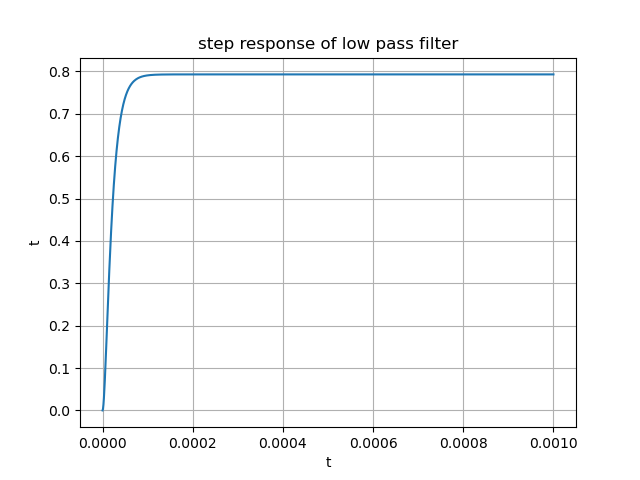
\includegraphics[scale = 1]{Figure_3.png}
    \caption{The step response in the time domain}
\end{figure}


\subsection{Question 2: Response to a Sum of Sinusoidal inputs}
Now, the input is given by:
\begin{equation}
    v_i(t) = (sin(2000*\pi*t) + cos(2*10^6*\pi*t))*u(t)
\end{equation}
so to find the output we use the \textbf{sp.lsim} command, which gives out the convolution of a given transfer function and input signal.

\subsubsection{Code:}

\begin{python}
#finding the solutoion matrix
A,b,V=lowpass(10000,10000,1e-9,1e-9,1.586,1)
Vo=V[3]
w=p.logspace(0,8,801)
ss=1j*w
hf=lambdify(s,Vo,'numpy')
v=hf(ss)
\end{python}

\begin{python}
#Question 2:

#getting the input signal
t = p.linspace(0,0.005,10000)
v_i = p.multiply(p.sin(2000*p.pi*t) + p.cos(2*1e6*p.pi*t),p.heaviside(t,0.5))

#getting the transfer function of the LPF
H2 = sympy_to_H_lti(Vo,s)

#performing the convolution
t,y,svec=sp.lsim(H2,v_i,t)
plot_display(t,y,'t','y','output response of input sinusoids','linear','linear')
\end{python}

\subsubsection{Output Signal}
\begin{figure}[H]
    \centering
    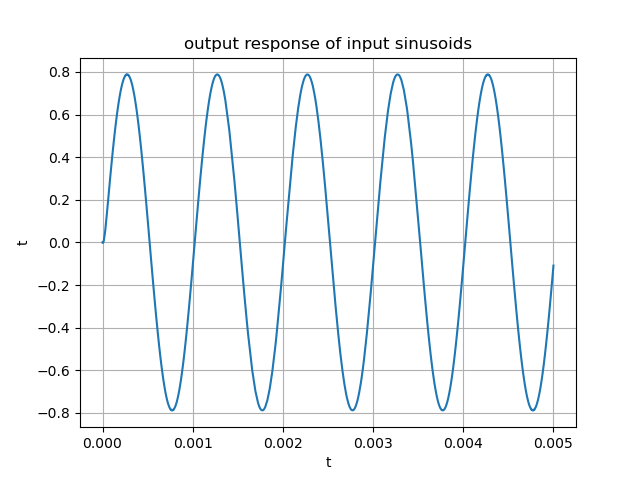
\includegraphics[scale = 1]{Figure_4.png}
    \caption{Response of the LPf with mixed sinusoidal signals}
\end{figure}

\subsection{Observations}
We can clearly see that the high frequency $10^6$Hz sinusoid gets filtered out leaving only the $10^3$Hz signal left.


\subsection{Question 3:}
This question has already been answered in the \textbf{The High Pass Filter} section near the beginning of this report.

\subsection{Question 4: Response of a Damped sinusoid}
We take 2 signals, first is a high freq, high decay coeff signal and the second is a low freq, high decay coeff signal.

\subsubsection{Code:}
\begin{python}
#Question 4:

#defining a function that gives the output as damped sinusoid
#with all the necessary input parameters
def damped_sinusoid(freq,type,decay,t):
	if type == 'sin':
		return p.sin(freq*2*p.pi*t)*p.exp(-1*decay*t)
	if type == 'cos':
		return p.cos(freq*2*p.pi*t)*p.exp(-1*decay*t)


#plotting the input and output graphs for a low freq, high decay sinusoid
t = p.linspace(0,0.01,10000)
v_i3 = damped_sinusoid(2000,'sin',1000,t)
t,y,svec=sp.lsim(H3,v_i3,t)
plot_display(t,damped_sinusoid(2000,'sin',1000,t),'t','$v_i3$','damped sinusoid input response (low freq)','linear','linear')
plot_display(t,y,'t','y','output response','linear','linear')


#plotting the input and output graphs for a high freq, high decay sinusoid
t = p.linspace(0,0.01,10000)
v_i4 = damped_sinusoid(20000,'sin',1000,t)
t,y,svec=sp.lsim(H3,v_i4,t)
plot_display(t,damped_sinusoid(20000,'sin',1000,t),'t','$v_i4$','damped sinusoid input response (high freq)','linear','linear')
plot_display(t,y,'t','y','output response','linear','linear')
\end{python}


\subsubsection{Signal 1}
for signal 1, 
\begin{equation}
    V_i(t) = (sin(2000*t))e^(^-^1^0^0^0^*^t^) * u(t)
\end{equation}

\subsubsection{Input of the low freq damped sinusoid}
\begin{figure}[H]
    \centering
    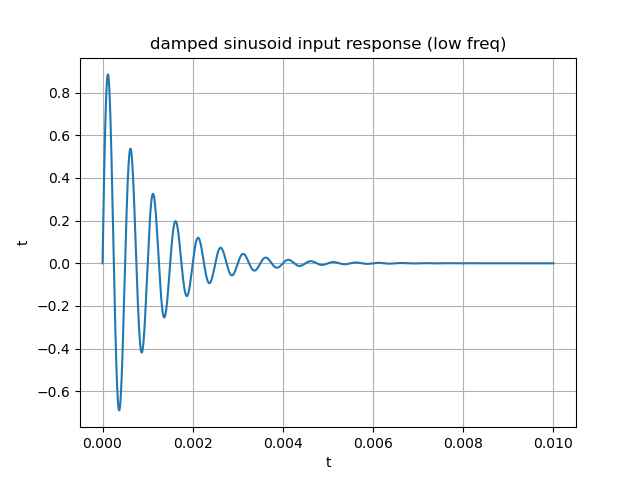
\includegraphics[scale = 1]{Figure_6.png}
    \caption{Low freq damped sinusoid}
\end{figure}

\subsubsection{Output of the Low freq damped sinusoid}
\begin{figure}[H]
    \centering
    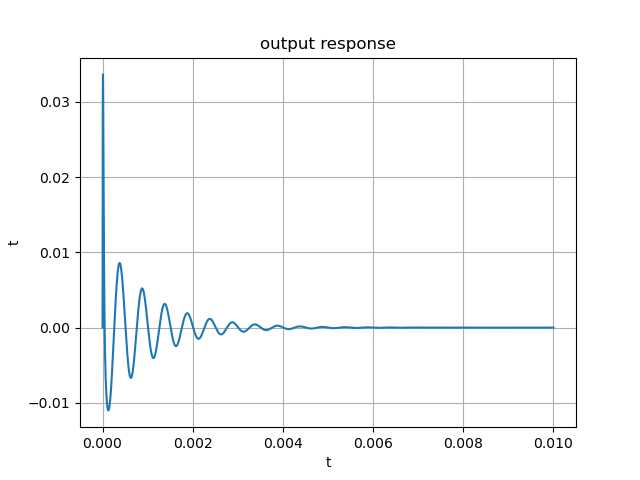
\includegraphics[scale = 1]{Figure_7.png}
    \caption{Output of the Low freq damped sinusoid}
\end{figure}


\subsection{Signal 2}
for signal 2, 
\begin{equation}
    V_i(t) = (sin(20000*t))e^(^-^1^0^0^0^*^t^) * u(t)
\end{equation}

\subsubsection{Input of the high freq damped sinusoid}
\begin{figure}[H]
    \centering
    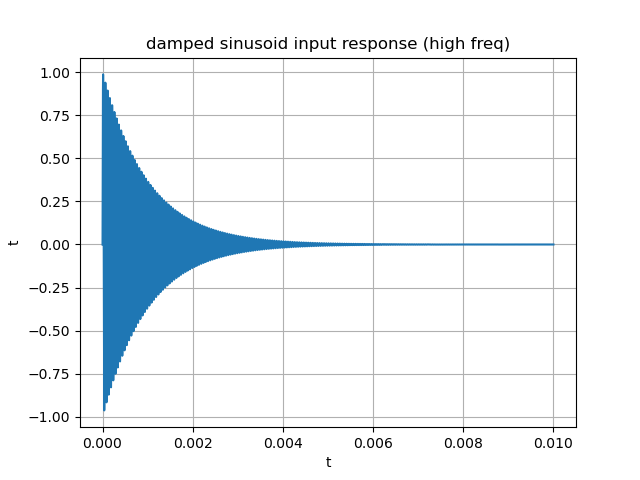
\includegraphics[scale = 1]{Figure_8.png}
    \caption{High freq damped sinusoid}
\end{figure}

\subsubsection{Output of the High freq damped sinusoid}
\begin{figure}[H]
    \centering
    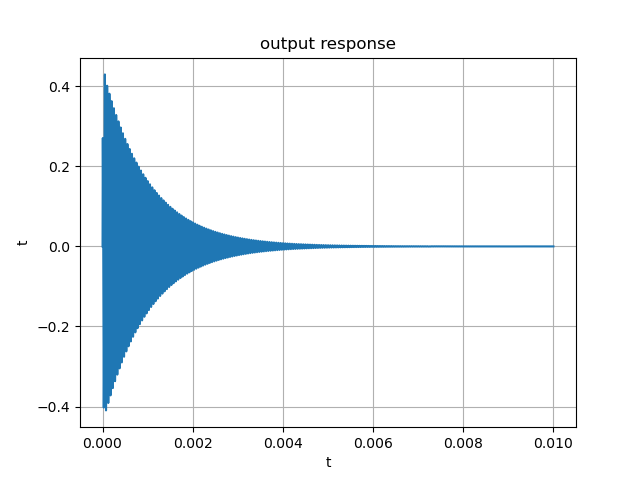
\includegraphics[scale = 1]{Figure_9.png}
    \caption{Output of the High freq damped sinusoid}
\end{figure}

\subsection{Question 5: Unit Step Response of the HPF}
The plots of the step response are given by:

\begin{figure}[H]
    \centering
    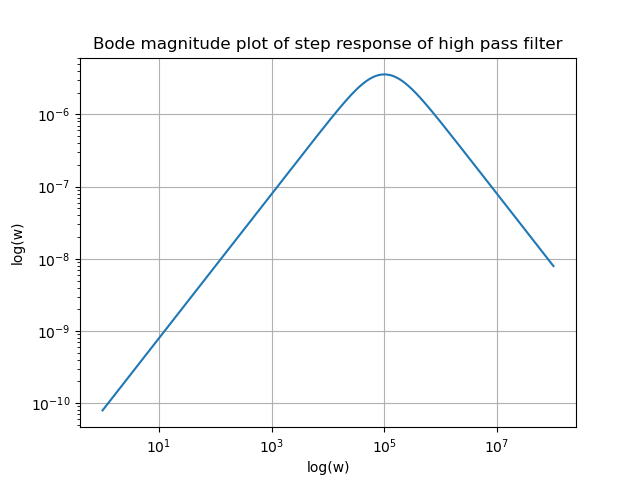
\includegraphics[scale = 1]{Figure_10.png}
    \caption{Bode magnitude plot of the Step Response}
\end{figure}

\begin{figure}[H]
    \centering
    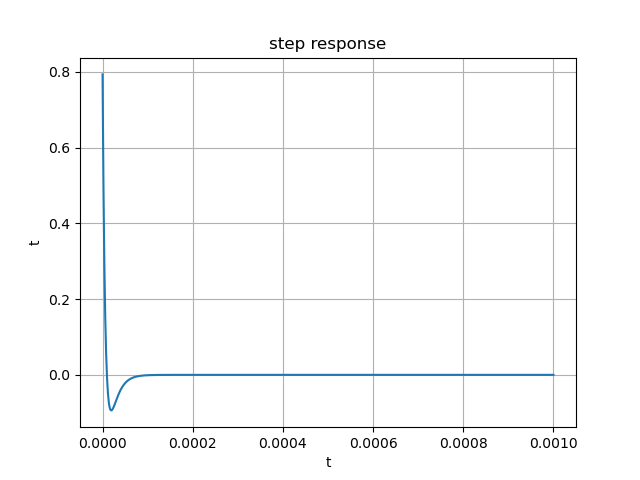
\includegraphics[scale = 1]{Figure_11.png}
    \caption{Plot of the Step Response}
\end{figure}

\subsubsection{Analysis of the response}
Initially, there is a jump in $V_o$ as the capacitors act like a short circuit just after the abrupt change in the input voltage, but as time goes on, the capacitors act like open circuits and the final output voltage drops to 0. 

\section{Conclusions}
In this assignment, we've learnt how to:
\begin{itemize}
    \item Analyse complicated circuits in the Laplace domain through nodal analysis
    \item Use the sympy library to obtain simplified versions of the transfer functions
    \item Converting expressions between sympy and other syntax's (such as numpy or scipy)
    \item obtaining the graphs of outputs and the respective bode plots
\end{itemize}









\end{document}
